
%
% 6.869 problem set 1
%
\documentclass[12pt,twoside]{article}

\usepackage{amsmath}
\usepackage{color}
\usepackage{clrscode}
\usepackage[pdftex]{graphicx}

% Cross-references for handout numbers.

% Updated to include SMA course for Fall 2001 -- cel

\newcommand{\name}{}


\usepackage{latexsym}
%\usepackage{bbm}
\usepackage{times,url}
\usepackage{clrscode}

\newcommand{\mitst}[1]{\begin{description}
\item[MIT students:] #1
\end{description}}
\newcommand{\smast}[1]{\begin{description}
\item[SMA students:] #1
\end{description}}

%\newcommand{\collabs}{Professors Srini Devadas, Nancy Lynch and Vinod Vaikuntanathan}
\newcommand{\subj}{6.006}

\newlength{\toppush}
\setlength{\toppush}{2\headheight}
\addtolength{\toppush}{\headsep}

\newcommand{\htitle}[2]{\noindent\vspace*{-\toppush}\newline\parbox{6.5in}
{\textit{6.869 Advances in Computer Vision}\hfill\name\newline
Andrew Moran \hfill #2\newline
\collabs\hfill #1 \vspace*{-.5ex}\newline
\mbox{}\hrulefill\mbox{}}\vspace*{1ex}\mbox{}\newline
\begin{center}{\Large\bf #1}\end{center}}

\newcommand{\handout}[2]{\thispagestyle{empty}
 \markboth{#1}{#1}
 \pagestyle{myheadings}\htitle{#1}{#2}}

\newcommand{\htitlewithouttitle}[2]{\noindent\vspace*{-\toppush}\newline\parbox{6.5in}
{\textit{Introduction to Algorithms}\hfill#2\newline
Massachusetts Institute of Technology \hfill 6.006\newline
%Singapore-MIT Alliance \hfill SMA5503\newline
\profs\hfill Handout #1\vspace*{-.5ex}\newline
\mbox{}\hrulefill\mbox{}}\vspace*{1ex}\mbox{}\newline}

\newcommand{\handoutwithouttitle}[2]{\thispagestyle{empty}
 \markboth{Handout \protect\ref{#1}}{Handout \protect\ref{#1}}
 \pagestyle{myheadings}\htitlewithouttitle{\protect\ref{#1}}{#2}}

\newcommand{\exam}[2]{% parameters: exam name, date
 \thispagestyle{empty}
 \markboth{\subj\ #1\hspace{1in}Name\hrulefill\ \ }%
          {\subj\ #1\hspace{1in}Name\hrulefill\ \ }
 \pagestyle{myheadings}\examtitle{#1}{#2}
 \renewcommand{\theproblem}{Problem \arabic{problemnum}}
}
\newcommand{\examsolutions}[3]{% parameters: handout, exam name, date
 \thispagestyle{empty}
 \markboth{Handout \protect\ref{#1}: #2}{Handout \protect\ref{#1}: #2}
% \pagestyle{myheadings}\htitle{\protect\ref{#1}}{#2}{#3}
 \pagestyle{myheadings}\examsolutionstitle{\protect\ref{#1}} {#2}{#3}
 \renewcommand{\theproblem}{Problem \arabic{problemnum}}
}
\newcommand{\examsolutionstitle}[3]{\noindent\vspace*{-\toppush}\newline\parbox{6.5in}
{\textit{Introduction to Algorithms}\hfill#3\newline
Massachusetts Institute of Technology \hfill 6.006\newline
%Singapore-MIT Alliance \hfill SMA5503\newline
\profs\hfill Handout #1\vspace*{-.5ex}\newline
\mbox{}\hrulefill\mbox{}}\vspace*{1ex}\mbox{}\newline
\begin{center}{\Large\bf #2}\end{center}}

\newcommand{\takehomeexam}[2]{% parameters: exam name, date
 \thispagestyle{empty}
 \markboth{\subj\ #1\hfill}{\subj\ #1\hfill}
 \pagestyle{myheadings}\examtitle{#1}{#2}
 \renewcommand{\theproblem}{Problem \arabic{problemnum}}
}

\makeatletter
\newcommand{\exambooklet}[2]{% parameters: exam name, date
 \thispagestyle{empty}
 \markboth{\subj\ #1}{\subj\ #1}
 \pagestyle{myheadings}\examtitle{#1}{#2}
 \renewcommand{\theproblem}{Problem \arabic{problemnum}}
 \renewcommand{\problem}{\newpage
 \item \let\@currentlabel=\theproblem
 \markboth{\subj\ #1, \theproblem}{\subj\ #1, \theproblem}}
}
\makeatother


\newcommand{\examtitle}[2]{\noindent\vspace*{-\toppush}\newline\parbox{6.5in}
{\textit{Introduction to Algorithms}\hfill#2\newline
Massachusetts Institute of Technology \hfill 6.006 Spring 2014\newline
%Singapore-MIT Alliance \hfill SMA5503\newline
\profs\hfill #1\vspace*{-.5ex}\newline
\mbox{}\hrulefill\mbox{}}\vspace*{1ex}\mbox{}\newline
\begin{center}{\Large\bf #1}\end{center}}

\newcommand{\grader}[1]{\hspace{1cm}\textsf{\textbf{#1}}\hspace{1cm}}

\newcommand{\points}[1]{[#1 points]\ }
\newcommand{\parts}[1]
{
  \ifnum#1=1
  (1 part)
  \else
  (#1 parts)
  \fi
  \ 
}

\newcommand{\bparts}{\begin{problemparts}}
\newcommand{\eparts}{\end{problemparts}}
\newcommand{\ppart}{\problempart}

%\newcommand{\lg} {lg\ }

\setlength{\oddsidemargin}{0pt}
\setlength{\evensidemargin}{0pt}
\setlength{\textwidth}{6.5in}
\setlength{\topmargin}{0in}
\setlength{\textheight}{8.5in}


\newcommand{\Spawn}{{\bf spawn} }
\newcommand{\Sync}{{\bf sync}}

\renewcommand{\cases}[1]{\left\{ \begin{array}{ll}#1\end{array}\right.}
\newcommand{\cif}[1]{\mbox{if $#1$}}
\newcommand{\cwhen}[1]{\mbox{when $#1$}}

\newcounter{problemnum}
\newcommand{\theproblem}{Problem \theproblemsetnum-\arabic{problemnum}}
\newenvironment{problems}{
        \begin{list}{{\bf \theproblem. \hspace*{0.5em}}}
        {\setlength{\leftmargin}{0em}
         \setlength{\rightmargin}{0em}
         \setlength{\labelwidth}{0em}
         \setlength{\labelsep}{0em}
         \usecounter{problemnum}}}{\end{list}}
\makeatletter
\newcommand{\problem}[1][{}]{\item \let\@currentlabel=\theproblem \textbf{#1}}
\makeatother

\newcounter{problempartnum}[problemnum]
\newenvironment{problemparts}{
        \begin{list}{{\bf (\alph{problempartnum})}}
        {\setlength{\leftmargin}{2.5em}
         \setlength{\rightmargin}{2.5em}
         \setlength{\labelsep}{0.5em}}}{\end{list}}
\newcommand{\problempart}{\addtocounter{problempartnum}{1}\item}

\newenvironment{truefalseproblemparts}{
        \begin{list}{{\bf (\alph{problempartnum})\ \ \ T\ \ F\hfil}}
        {\setlength{\leftmargin}{4.5em}
         \setlength{\rightmargin}{2.5em}
         \setlength{\labelsep}{0.5em}
         \setlength{\labelwidth}{4.5em}}}{\end{list}}

\newcounter{exercisenum}
\newcommand{\theexercise}{Exercise \theproblemsetnum-\arabic{exercisenum}}
\newenvironment{exercises}{
        \begin{list}{{\bf \theexercise. \hspace*{0.5em}}}
        {\setlength{\leftmargin}{0em}
         \setlength{\rightmargin}{0em}
         \setlength{\labelwidth}{0em}
         \setlength{\labelsep}{0em}
        \usecounter{exercisenum}}}{\end{list}}
\makeatletter
\newcommand{\exercise}{\item \let\@currentlabel=\theexercise}
\makeatother

\newcounter{exercisepartnum}[exercisenum]
%\newcommand{\problem}[1]{\medskip\mbox{}\newline\noindent{\bf Problem #1.}\hspace*{1em}}
%\newcommand{\exercise}[1]{\medskip\mbox{}\newline\noindent{\bf Exercise #1.}\hspace*{1em}}

\newenvironment{exerciseparts}{
        \begin{list}{{\bf (\alph{exercisepartnum})}}
        {\setlength{\leftmargin}{2.5em}
         \setlength{\rightmargin}{2.5em}
         \setlength{\labelsep}{0.5em}}}{\end{list}}
\newcommand{\exercisepart}{\addtocounter{exercisepartnum}{1}\item}


% Macros to make captions print with small type and 'Figure xx' in bold.
\makeatletter
\def\fnum@figure{{\bf Figure \thefigure}}
\def\fnum@table{{\bf Table \thetable}}
\let\@mycaption\caption
%\long\def\@mycaption#1[#2]#3{\addcontentsline{\csname
%  ext@#1\endcsname}{#1}{\protect\numberline{\csname 
%  the#1\endcsname}{\ignorespaces #2}}\par
%  \begingroup
%    \@parboxrestore
%    \small
%    \@makecaption{\csname fnum@#1\endcsname}{\ignorespaces #3}\par
%  \endgroup}
%\def\mycaption{\refstepcounter\@captype \@dblarg{\@mycaption\@captype}}
%\makeatother
\let\mycaption\caption
%\newcommand{\figcaption}[1]{\mycaption[]{#1}}

\newcounter{totalcaptions}
\newcounter{totalart}

\newcommand{\figcaption}[1]{\addtocounter{totalcaptions}{1}\caption[]{#1}}

% \psfigures determines what to do for figures:
%       0 means just leave vertical space
%       1 means put a vertical rule and the figure name
%       2 means insert the PostScript version of the figure
%       3 means put the figure name flush left or right
\newcommand{\psfigures}{0}
\newcommand{\spacefigures}{\renewcommand{\psfigures}{0}}
\newcommand{\rulefigures}{\renewcommand{\psfigures}{1}}
\newcommand{\macfigures}{\renewcommand{\psfigures}{2}}
\newcommand{\namefigures}{\renewcommand{\psfigures}{3}}

\newcommand{\figpart}[1]{{\bf (#1)}\nolinebreak[2]\relax}
\newcommand{\figparts}[2]{{\bf (#1)--(#2)}\nolinebreak[2]\relax}


\macfigures     % STATE

% When calling \figspace, make sure to leave a blank line afterward!!
% \widefigspace is for figures that are more than 28pc wide.
\newlength{\halffigspace} \newlength{\wholefigspace}
\newlength{\figruleheight} \newlength{\figgap}
\newcommand{\setfiglengths}{\ifnum\psfigures=1\setlength{\figruleheight}{\hruleheight}\setlength{\figgap}{1em}\else\setlength{\figruleheight}{0pt}\setlength{\figgap}{0em}\fi}
\newcommand{\figspace}[2]{\ifnum\psfigures=0\leavefigspace{#1}\else%
\setfiglengths%
\setlength{\wholefigspace}{#1}\setlength{\halffigspace}{.5\wholefigspace}%
\rule[-\halffigspace]{\figruleheight}{\wholefigspace}\hspace{\figgap}#2\fi}
\newlength{\widefigspacewidth}
% Make \widefigspace put the figure flush right on the text page.
\newcommand{\widefigspace}[2]{
\ifnum\psfigures=0\leavefigspace{#1}\else%
\setfiglengths%
\setlength{\widefigspacewidth}{28pc}%
\addtolength{\widefigspacewidth}{-\figruleheight}%
\setlength{\wholefigspace}{#1}\setlength{\halffigspace}{.5\wholefigspace}%
\makebox[\widefigspacewidth][r]{#2\hspace{\figgap}}\rule[-\halffigspace]{\figruleheight}{\wholefigspace}\fi}
\newcommand{\leavefigspace}[1]{\setlength{\wholefigspace}{#1}\setlength{\halffigspace}{.5\wholefigspace}\rule[-\halffigspace]{0em}{\wholefigspace}}

% Commands for including figures with macpsfig.
% To use these commands, documentstyle ``macpsfig'' must be specified.
\newlength{\macfigfill}
\makeatother
\newlength{\bbx}
\newlength{\bby}
\newcommand{\macfigure}[5]{\addtocounter{totalart}{1}
\ifnum\psfigures=2%
\setlength{\bbx}{#2}\addtolength{\bbx}{#4}%
\setlength{\bby}{#3}\addtolength{\bby}{#5}%
\begin{flushleft}
\ifdim#4>28pc\setlength{\macfigfill}{#4}\addtolength{\macfigfill}{-28pc}\hspace*{-\macfigfill}\fi%
\mbox{\psfig{figure=./#1.ps,%
bbllx=#2,bblly=#3,bburx=\bbx,bbury=\bby}}
\end{flushleft}%
\else\ifdim#4>28pc\widefigspace{#5}{#1}\else\figspace{#5}{#1}\fi\fi}
\makeatletter

\newlength{\savearraycolsep}
\newcommand{\narrowarray}[1]{\setlength{\savearraycolsep}{\arraycolsep}\setlength{\arraycolsep}{#1\arraycolsep}}
\newcommand{\normalarray}{\setlength{\arraycolsep}{\savearraycolsep}}

\newcommand{\hint}{{\em Hint:\ }}

% Macros from /th/u/clr/mac.tex

\newcommand{\set}[1]{\left\{ #1 \right\}}
\newcommand{\abs}[1]{\left| #1\right|}
\newcommand{\card}[1]{\left| #1\right|}
\newcommand{\floor}[1]{\left\lfloor #1 \right\rfloor}
\newcommand{\ceil}[1]{\left\lceil #1 \right\rceil}
\newcommand{\ang}[1]{\ifmmode{\left\langle #1 \right\rangle}
   \else{$\left\langle${#1}$\right\rangle$}\fi}
        % the \if allows use outside mathmode,
        % but will swallow following space there!
\newcommand{\paren}[1]{\left( #1 \right)}
\newcommand{\bracket}[1]{\left[ #1 \right]}
\newcommand{\prob}[1]{\Pr\left\{ #1 \right\}}
\newcommand{\Var}{\mathop{\rm Var}\nolimits}
\newcommand{\expect}[1]{{\rm E}\left[ #1 \right]}
\newcommand{\expectsq}[1]{{\rm E}^2\left[ #1 \right]}
\newcommand{\variance}[1]{{\rm Var}\left[ #1 \right]}
\renewcommand{\choose}[2]{{{#1}\atopwithdelims(){#2}}}
\def\pmod#1{\allowbreak\mkern12mu({\rm mod}\,\,#1)}
\newcommand{\matx}[2]{\left(\begin{array}{*{#1}{c}}#2\end{array}\right)}
\newcommand{\Adj}{\mathop{\rm Adj}\nolimits}

\newtheorem{theorem}{Theorem}
\newtheorem{lemma}[theorem]{Lemma}
\newtheorem{corollary}[theorem]{Corollary}
\newtheorem{xample}{Example}
\newtheorem{definition}{Definition}
\newenvironment{example}{\begin{xample}\rm}{\end{xample}}
\newcommand{\proof}{\noindent{\em Proof.}\hspace{1em}}
\def\squarebox#1{\hbox to #1{\hfill\vbox to #1{\vfill}}}
\newcommand{\qedbox}{\vbox{\hrule\hbox{\vrule\squarebox{.667em}\vrule}\hrule}}
\newcommand{\qed}{\nopagebreak\mbox{}\hfill\qedbox\smallskip}
\newcommand{\eqnref}[1]{(\protect\ref{#1})}

%%\newcommand{\twodots}{\mathinner{\ldotp\ldotp}}
\newcommand{\transpose}{^{\mbox{\scriptsize \sf T}}}
\newcommand{\amortized}[1]{\widehat{#1}}

\newcommand{\punt}[1]{}

%%% command for putting definitions into boldface
% New style for defined terms, as of 2/23/88, redefined by THC.
\newcommand{\defn}[1]{{\boldmath\textit{\textbf{#1}}}}
\newcommand{\defi}[1]{{\textit{\textbf{#1\/}}}}

\newcommand{\red}{\leq_{\rm P}}
\newcommand{\lang}[1]{%
\ifmmode\mathord{\mathcode`-="702D\rm#1\mathcode`\-="2200}\else{\rm#1}\fi}

%\newcommand{\ckt}[1]{\ifmmode\mathord{\mathcode`-="702D\sc #1\mathcode`\-="2200}\else$\mathord{\mathcode`-="702D\sc #1\mathcode`\-="2200}$\fi}
\newcommand{\ckt}[1]{\ifmmode \sc #1\else$\sc #1$\fi}

%% Margin notes - use \notesfalse to turn off notes.
\setlength{\marginparwidth}{0.6in}
\reversemarginpar
\newif\ifnotes
\notestrue
\newcommand{\longnote}[1]{
  \ifnotes
    {\medskip\noindent Note: \marginpar[\hfill$\Longrightarrow$]
      {$\Longleftarrow$}{#1}\medskip}
  \fi}
\newcommand{\note}[1]{
  \ifnotes
    {\marginpar{\tiny \raggedright{#1}}}
  \fi}


\newcommand{\reals}{\mathbbm{R}}
\newcommand{\integers}{\mathbbm{Z}}
\newcommand{\naturals}{\mathbbm{N}}
\newcommand{\rationals}{\mathbbm{Q}}
\newcommand{\complex}{\mathbbm{C}}

\newcommand{\oldreals}{{\bf R}}
\newcommand{\oldintegers}{{\bf Z}}
\newcommand{\oldnaturals}{{\bf N}}
\newcommand{\oldrationals}{{\bf Q}}
\newcommand{\oldcomplex}{{\bf C}}

\newcommand{\w}{\omega}                 %% for fft chapter

\newenvironment{closeitemize}{\begin{list}
{$\bullet$}
{\setlength{\itemsep}{-0.2\baselineskip}
\setlength{\topsep}{0.2\baselineskip}
\setlength{\parskip}{0pt}}}
{\end{list}}

% These are necessary within a {problems} environment in order to restore
% the default separation between bullets and items.
\newenvironment{normalitemize}{\setlength{\labelsep}{0.5em}\begin{itemize}}
                              {\end{itemize}}
\newenvironment{normalenumerate}{\setlength{\labelsep}{0.5em}\begin{enumerate}}
                                {\end{enumerate}}

%\def\eqref#1{Equation~(\ref{eq:#1})}
%\newcommand{\eqref}[1]{Equation (\ref{eq:#1})}
\newcommand{\eqreftwo}[2]{Equations (\ref{eq:#1}) and~(\ref{eq:#2})}
\newcommand{\ineqref}[1]{Inequality~(\ref{ineq:#1})}
\newcommand{\ineqreftwo}[2]{Inequalities (\ref{ineq:#1}) and~(\ref{ineq:#2})}

\newcommand{\figref}[1]{Figure~\ref{fig:#1}}
\newcommand{\figreftwo}[2]{Figures \ref{fig:#1} and~\ref{fig:#2}}

\newcommand{\liref}[1]{line~\ref{li:#1}}
\newcommand{\Liref}[1]{Line~\ref{li:#1}}
\newcommand{\lirefs}[2]{lines \ref{li:#1}--\ref{li:#2}}
\newcommand{\Lirefs}[2]{Lines \ref{li:#1}--\ref{li:#2}}
\newcommand{\lireftwo}[2]{lines \ref{li:#1} and~\ref{li:#2}}
\newcommand{\lirefthree}[3]{lines \ref{li:#1}, \ref{li:#2}, and~\ref{li:#3}}

\newcommand{\lemlabel}[1]{\label{lem:#1}}
\newcommand{\lemref}[1]{Lemma~\ref{lem:#1}} 

\newcommand{\exref}[1]{Exercise~\ref{ex:#1}}

\newcommand{\handref}[1]{Handout~\ref{#1}}

\newcommand{\defref}[1]{Definition~\ref{def:#1}}

% (1997.8.16: Victor Luchangco)
% Modified \hlabel to only get date and to use handouts counter for number.
%   New \handout and \handoutwithouttitle commands in newmac.tex use this.
%   The date is referenced by <label>-date.
%   (Retained old definition as \hlabelold.)
%   Defined \hforcelabel to use an argument instead of the handouts counter.

\newcounter{handouts}
\setcounter{handouts}{0}

\newcommand{\hlabel}[2]{%
\stepcounter{handouts}
{\edef\next{\write\@auxout{\string\newlabel{#1}{{\arabic{handouts}}{0}}}}\next}
\write\@auxout{\string\newlabel{#1-date}{{#2}{0}}}
}

\newcommand{\hforcelabel}[3]{%          Does not step handouts counter.
\write\@auxout{\string\newlabel{#1}{{#2}{0}}}
\write\@auxout{\string\newlabel{#1-date}{{#3}{0}}}}


% less ugly underscore
% --juang, 2008 oct 05
\renewcommand{\_}{\vrule height 0 pt depth 0.4 pt width 0.5 em \,}


\setlength{\oddsidemargin}{0pt}
\setlength{\evensidemargin}{0pt}
\setlength{\textwidth}{6.5in}
\setlength{\topmargin}{0in}
\setlength{\textheight}{8.5in}

\newcommand{\theproblemsetnum}{2}
\newcommand{\partaduedate}{Sept 18, 2014 (1:00pm)}
\newcommand{\collabs}{Collaborators: None}
\newcommand{\tabUnit}{3ex}
\newcommand{\tabT}{\hspace*{\tabUnit}}

\title{6.869 PSET 2}

\begin{document}

\handout{Problem Set \theproblemsetnum}{Sept 18, 2014 (1:00pm)}
\tabT Resources with corresponding images and code are on Stellar under \texttt{andrewmo@mit.edu}.  The files are in the \texttt{pset2.zip} folder.  To reproduce the below figures, run \texttt{pset2main.m}.

\section*{Problem 2.1}
\tabT \textbf{(A)} Below are the laplacian pyramid decompositions broken up into 3 separate channels of the apple rgb image as the source image.  As you can tell, it reconstructs to the original image.
\newline

\tabT\tabT\tabT\tabT\tabT\tabT\tabT\tabT\tabT \textbf{Input}
\tabT\tabT\tabT\tabT\tabT\tabT\tabT \textbf{Output}

\DeclareGraphicsExtensions{.pdf,.png,.jpg}
\tabT\tabT\tabT\tabT\tabT
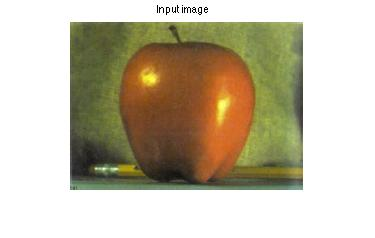
\includegraphics[width = 150pt, trim = 0pt 50pt 0pt 0pt, clip]{appleInput}
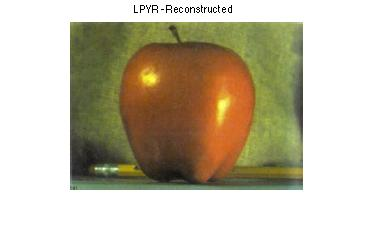
\includegraphics[width = 150pt, trim = 0pt 50pt 0pt 0pt, clip]{appleOutput}

\tabT\tabT\tabT \textbf{LPyr}: Red
\tabT\tabT\tabT\tabT\tabT\tabT \textbf{LPyr}: Green
\tabT\tabT\tabT\tabT\tabT \textbf{LPyr}: Blue

\DeclareGraphicsExtensions{.pdf,.png,.jpg}
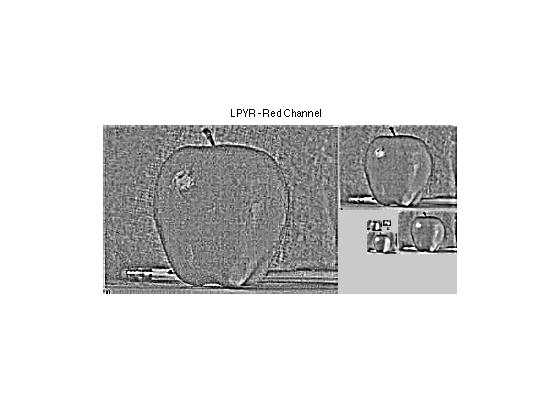
\includegraphics[width = 150pt, trim = 100pt 100pt 100pt 100pt, clip]{appleLR}
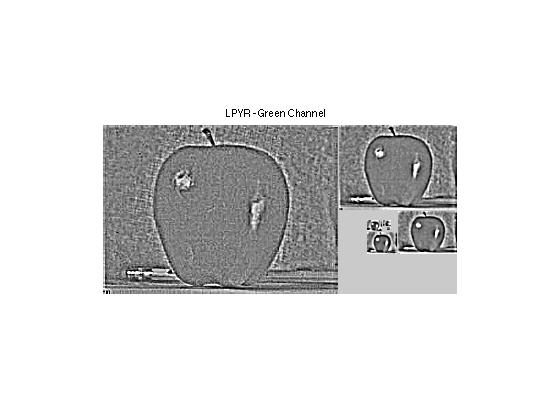
\includegraphics[width = 150pt, trim = 100pt 100pt 100pt 100pt, clip]{appleLG}
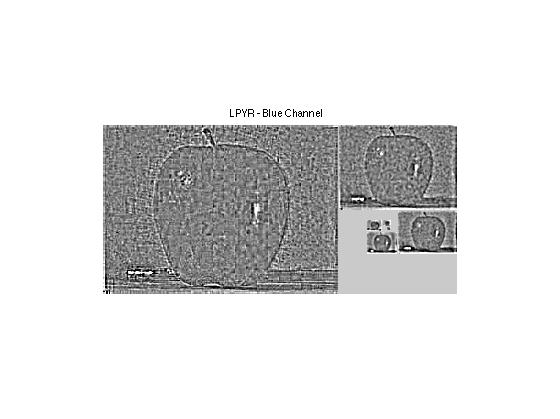
\includegraphics[width = 150pt, trim = 100pt 100pt 100pt 100pt, clip]{appleLB}
\newline

\tabT \textbf{(B)} Below are the source images, their Laplacian pyramids, blending mask, and resulting blended image.
\newline

\tabT\tabT\tabT\tabT\tabT\tabT\tabT\tabT\tabT \textbf{IM1}
\tabT\tabT\tabT\tabT\tabT\tabT\tabT \textbf{IM2}
\newline

\DeclareGraphicsExtensions{.pdf,.png,.jpg}
\tabT\tabT\tabT\tabT\tabT

\includegraphics[width = 150pt]{andremo_pic}
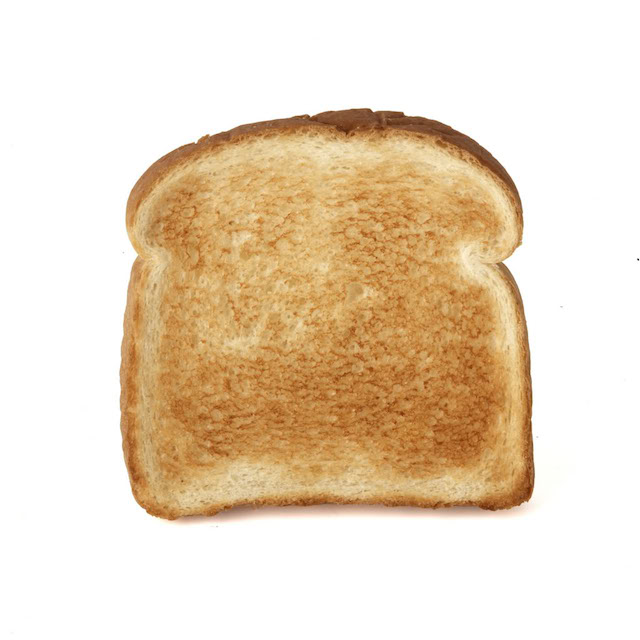
\includegraphics[width = 150pt]{toast}
\newline

\tabT\tabT\textbf{IM1 LPyr}: Red
\tabT\tabT\tabT\tabT \textbf{IM1 LPyr}: Green
\tabT\tabT\tabT\tabT \textbf{IM1 LPyr}: Blue

\DeclareGraphicsExtensions{.pdf,.png,.jpg}
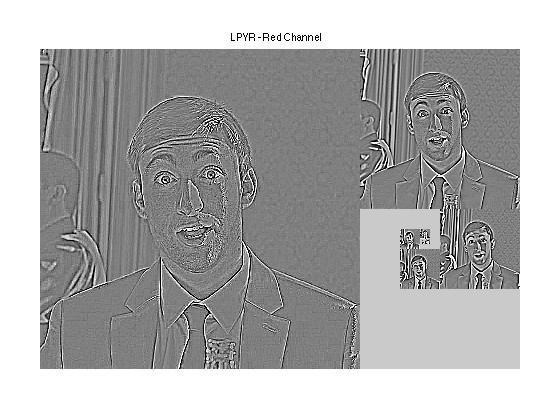
\includegraphics[width = 150pt]{andremo_lpyr_r}
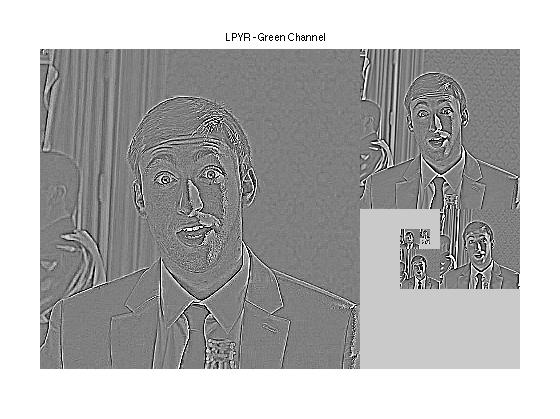
\includegraphics[width = 150pt]{andremo_lpyr_g}
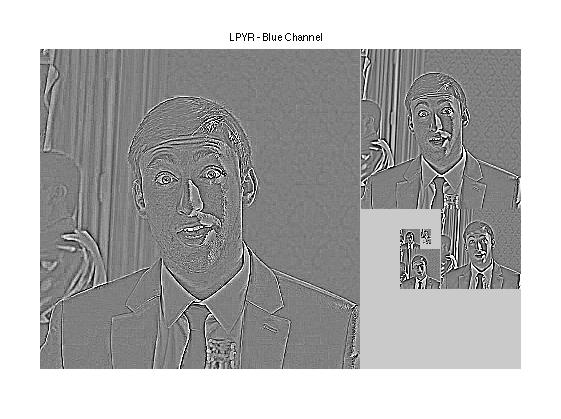
\includegraphics[width = 150pt]{andremo_lpyr_b}

\tabT\tabT \textbf{IM2 LPyr}: Red
\tabT\tabT\tabT\tabT \textbf{IM2 LPyr}: Green
\tabT\tabT\tabT\tabT \textbf{IM2 LPyr}: Blue

\DeclareGraphicsExtensions{.pdf,.png,.jpg}
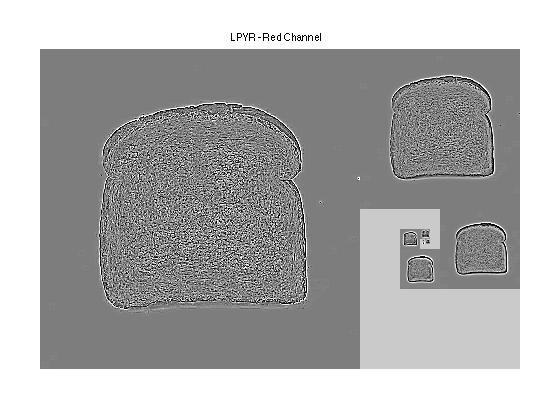
\includegraphics[width = 150pt]{toast_lpyr_r}
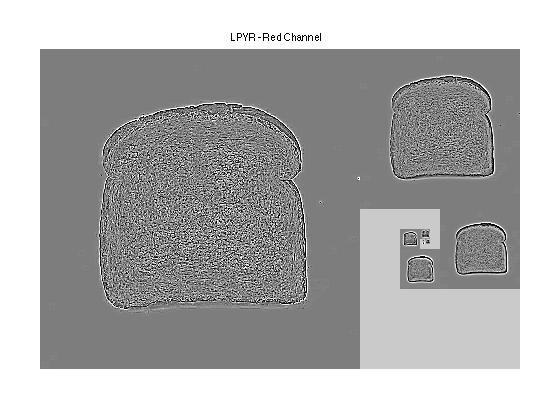
\includegraphics[width = 150pt]{toast_lpyr_r}
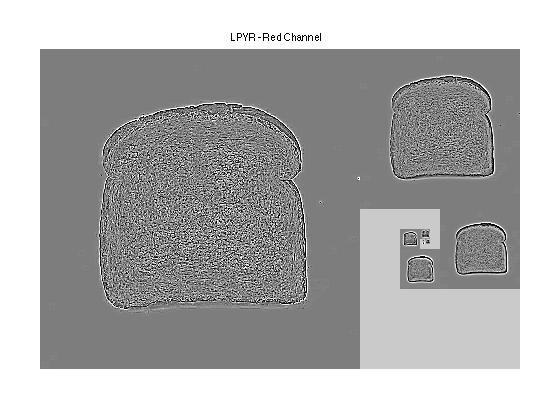
\includegraphics[width = 150pt]{toast_lpyr_r}

\tabT\tabT\tabT\tabT\tabT\tabT\tabT\tabT\tabT \textbf{Mask}
\tabT\tabT\tabT\tabT\tabT\tabT\tabT \textbf{Output}

\DeclareGraphicsExtensions{.pdf,.png,.jpg}
\tabT\tabT\tabT\tabT\tabT
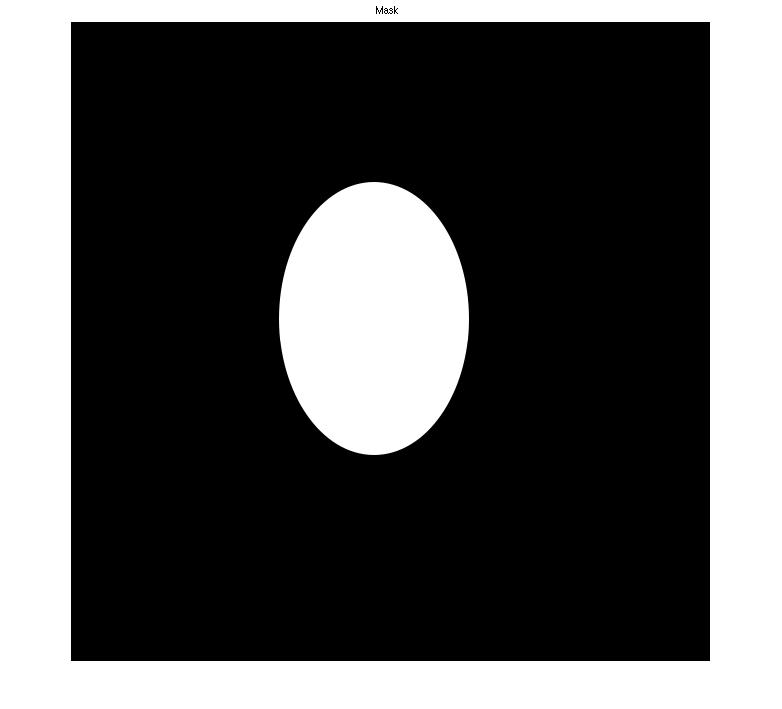
\includegraphics[width = 150pt]{lmask}
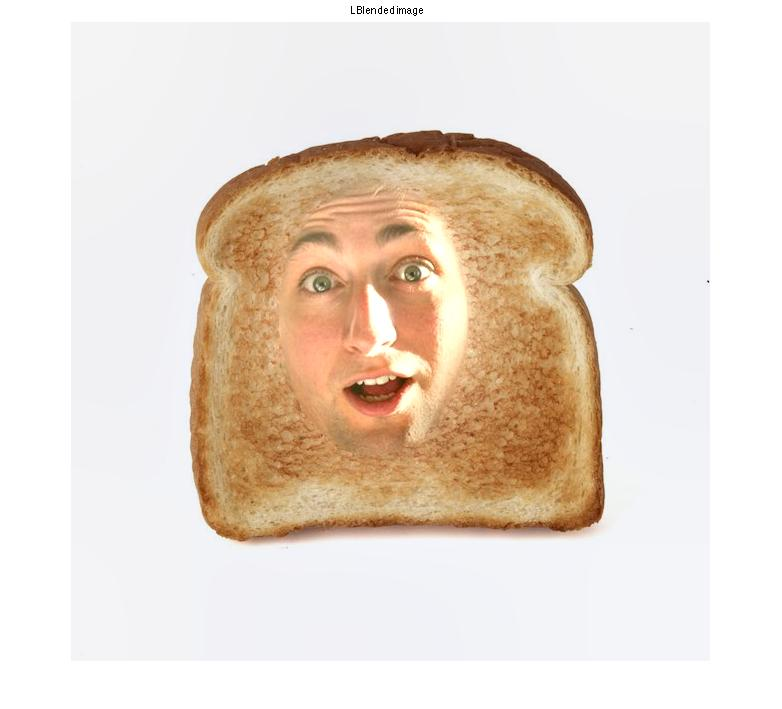
\includegraphics[width = 150pt]{lblended_image}


\section*{Problem 2.2}
\tabT Below are the source images, the resulting hybrid image, and a blurred version at level 3 of the pyramid.  Following the SIGGRAPH paper, I worked in in the frequency domain to manipulate the images with specific low/high cutoff frequencies.  The original closer image has the husky most prominent, however, the farther away you are from the image and more blurred it is, the face is more prominent.
\newline

\DeclareGraphicsExtensions{.pdf,.png,.jpg}
\hspace*{-20pt}
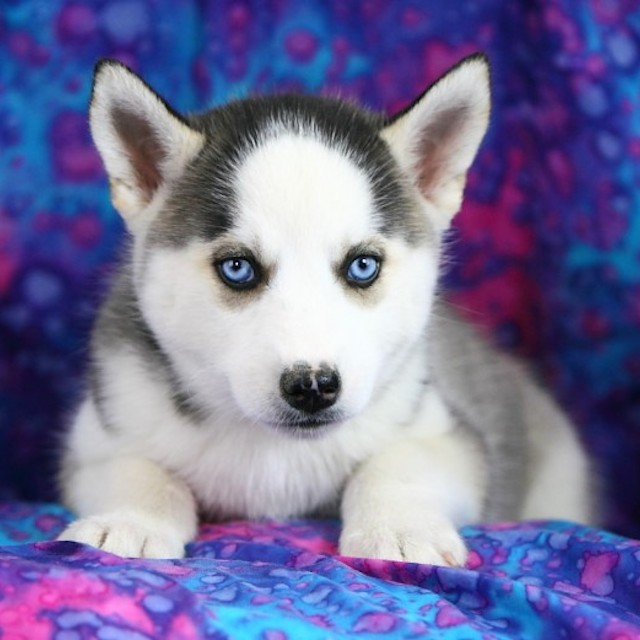
\includegraphics[width = 120pt, trim = 0pt 0pt 0pt 0pt, clip]{husky}

\includegraphics[width = 120pt]{andremo_pic}
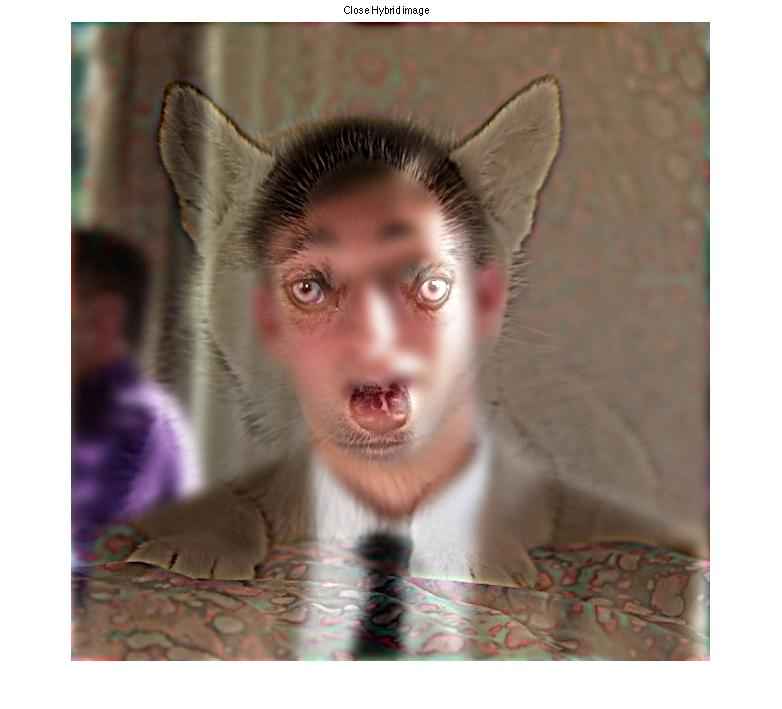
\includegraphics[scale = .27, trim = 75pt 50pt 75pt 0pt, clip]{close_hybrid_image}
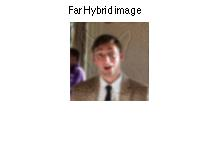
\includegraphics[scale = .7, trim = 75pt 50pt 20pt 20pt, clip]{far_hybrid_image}
\newline
\tabT\tabT\tabT \textbf{IMA}
\tabT\tabT\tabT\tabT\tabT\tabT \textbf{IMB}
\tabT\tabT\tabT\tabT\tabT\tabT\tabT \textbf{CLOSE}
\tabT\tabT\tabT\tabT \textbf{FAR}


\section*{Problem 2.3}
\tabT \textbf{(A)(i)} Prove $f \ast g = g \ast f$: (Convolution is commutative)
\newline
\newline
\tabT\tabT\tabT Use change of variable, let $j=t-j$. \newline
\tabT\tabT\tabT\tabT\tabT\tabT\tabT
$(f \ast g)[t] = \sum_{j=-\infty}^{\infty}f[t-j]g[j]$ \newline
\tabT\tabT\tabT\tabT\tabT\tabT\tabT\tabT\tabT\tabT
$= \sum_{j=\infty}^{-\infty}f[j]g[t-j]$ \newline
\tabT\tabT\tabT\tabT\tabT\tabT\tabT\tabT\tabT\tabT
$= \sum_{j=-\infty}^{\infty}g[t-j]f[j]$ \newline
\tabT\tabT\tabT\tabT\tabT\tabT\tabT\tabT\tabT\tabT
$= (g \ast f)[t]$ \newline

\textbf{(ii)} Prove $(f \ast g) \ast h = f \ast (g \ast h)$: (Convolution is associative) \newline
\newline
\tabT\tabT\tabT\tabT\tabT\tabT
$f \ast (g \ast h)[t] = f[t] \ast (\sum_{j=-\infty}^{\infty}g[t-j]h[j])$ \newline
\tabT\tabT\tabT\tabT\tabT\tabT\tabT\tabT\tabT\tabT
$= \sum_{k=-\infty}^{\infty} f[k] (\sum_{j=-\infty}^{\infty}g[t-k-j]h[j])$ \newline
\tabT\tabT\tabT\tabT\tabT\tabT\tabT\tabT\tabT\tabT
$= \sum_{k=-\infty}^{\infty} \sum_{j=-\infty}^{\infty} f[k]g[t-k-j]h[j])$, Let $j=j-k$ \newline
\tabT\tabT\tabT\tabT\tabT\tabT\tabT\tabT\tabT\tabT
$= \sum_{k=-\infty}^{\infty} \sum_{j=-\infty}^{\infty} f[k]g[j-k]h[t-j])$ \newline
\tabT\tabT\tabT\tabT\tabT\tabT\tabT\tabT\tabT\tabT
$= \sum_{j=-\infty}^{\infty} (\sum_{k=-\infty}^{\infty} f[k]g[j-k])h[t-j])$ \newline
\tabT\tabT\tabT\tabT\tabT\tabT\tabT\tabT\tabT\tabT
$= \sum_{j=-\infty}^{\infty} (f \ast g[j]) h[t-j])$ \newline
\tabT\tabT\tabT\tabT\tabT\tabT\tabT\tabT\tabT\tabT
$= (f \ast g) \ast h[t]$ \newline

\textbf{(iii)} Show that if $f$ is separable, then the 2D convolution $G \ast f$ can be computed as a sequence of two 1D convolutions. \newline
\newline
\tabT\tabT\tabT\tabT\tabT\tabT
Since $f=uv^{T}$, it is separable to $f_{1}$ of size (U x 1) and $f_{2}$ of size (1 x V) \newline
\tabT\tabT\tabT\tabT\tabT\tabT
$G \ast f[u,v] = \sum_{j=-\infty}^{\infty} \sum_{i=-\infty}^{\infty} G[i,j]f[u-i,v-j]$ \newline
\tabT\tabT\tabT\tabT\tabT\tabT\tabT\tabT\tabT
$= \sum_{j=-\infty}^{\infty} \sum_{i=-\infty}^{\infty} f[i,j]G[u-i,v-j]$, by commutativity \newline
\tabT\tabT\tabT\tabT\tabT\tabT\tabT\tabT\tabT
$= \sum_{j=-\infty}^{\infty} \sum_{i=-\infty}^{\infty} f_{1}[i]f_{2}[j]G[u-i,v-j]$, by separability \newline
\tabT\tabT\tabT\tabT\tabT\tabT\tabT\tabT\tabT
$= \sum_{j=-\infty}^{\infty} f_{2}[j] (\sum_{i=-\infty}^{\infty} f_{1}[i]G[u-i,v-j])$ \newline
\tabT\tabT\tabT\tabT\tabT\tabT\tabT\tabT\tabT
$= \sum_{j=-\infty}^{\infty} f_{2}[j] (f_{1}[i] \ast G[u-i,v-j])$ \newline
\tabT\tabT\tabT\tabT\tabT\tabT\tabT\tabT\tabT
$= f_{2}[j] \ast f_{1}[i] \ast G[u-i,v-j]$ \newline
\newline
Above shows that separable 2D convolution is a sequence of two 1D convultions (one vertically, one horizontally) and can be performed in any order due to the proof of associativity.
\newline
\newline

\textbf{(B)} Match the images to the log of the magnitude of their Fourier Transform.
\newline
\newline
\tabT \textbf{(1):D}
\newline
\tabT The brick wall is a grid with vertical and horizontal lines, however, the horizontal lines are more consistent/unform than the vertical lines.  Therefore, the FFT will have a magnitude where the vertical more prominent than the horizontal.
\newline 
\tabT \textbf{(2):A}
\newline
\tabT The grass is very uniform with no fine edges.  Therefore the FFT will be uniform as well.  The FT magnitude will be the highest in the center but decrease radially outwards.
\newline 
\tabT \textbf{(3):C}
\newline
\tabT The rocks are organized in a loose grid with fine edges.  Because the rocks have a generally round shape, they would have a FFT that radially decreases from the center.  The fine edges show prominence in the vertical and horizontal directions of the FFT.
\newline 
\tabT \textbf{(4):B}
\newline
\tabT The street light and wire are angled which is noticable in its FFT.  The pole is angled about 75 degress from the horizontal and the wire/light is angled about -45 degress from teh horizontal.  Image B shows the strongest magnitides at the 75 degrees from the vertical and -45 degrees from the vertical. 
\newline 
\tabT \textbf{(5):E}
\newline
\tabT The honeycomb grid is very organized and has constistency along multiple directions.  There are fine adges that go along the vertical and horizontal directions.  However, the shape of each honeycomb is consistent with symmtrical sides (some angled 45 from the vertical and horizontal axiis).  Therefore the FFT will show a strong magnitude in the vertical/horizontal driections, as well as the 45 degrees from both axiis.  This is depicted in Image E.
\newline

\section*{Problem 2.4}
\tabT Steerable filters as decribed by Freeman and Adelson.  There may be slight deviation when comparing my images to the staff's due to choice of epsilon.  Using Einstein's portrait as input, the below figures show G2 steered in the dominant and perpendicular directions (original, normalized, mean-filtered). 
\newline

\DeclareGraphicsExtensions{.pdf,.png,.jpg}
\tabT\tabT \textbf{INPUT}
\tabT\tabT\tabT\tabT\tabT\tabT \textbf{G2}: dominant
\tabT\tabT\tabT\tabT\tabT\tabT \textbf{G2}: perpedicular
\newline
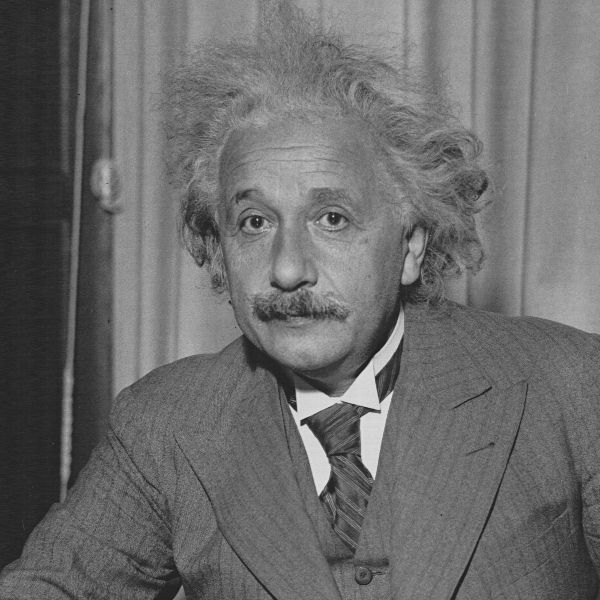
\includegraphics[scale = .2, trim = 0pt -130pt 0pt 0pt, clip]{einstein}
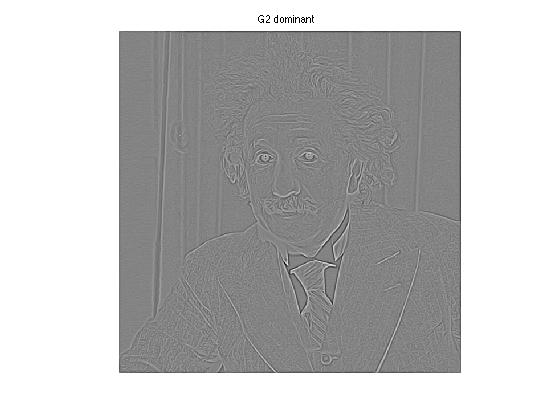
\includegraphics[width = 168pt, trim = 80pt 20pt 100pt 30pt, clip]{G2d}
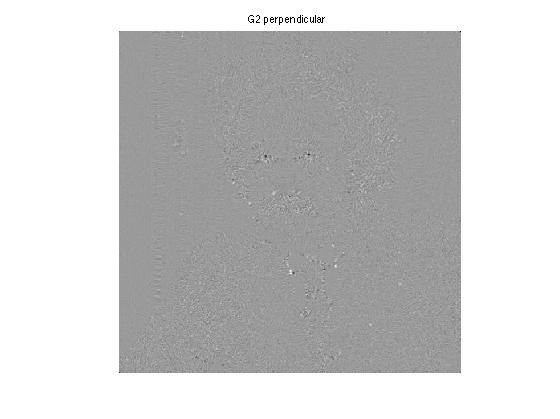
\includegraphics[width = 168pt, trim = 80pt 20pt 100pt 30pt, clip]{G2p}
\newline
\tabT\tabT\tabT\tabT\tabT\tabT\tabT
\tabT\tabT\tabT\tabT \textbf{G2}: dominant norm
\tabT\tabT\tabT\tabT \textbf{G2}: perpedicular norm
\newline
\tabT\tabT\tabT\tabT\tabT\tabT\tabT\tabT
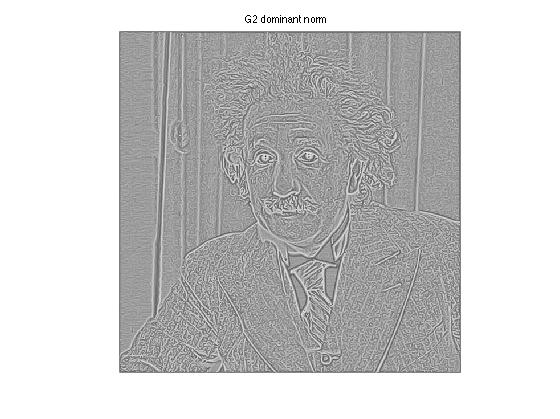
\includegraphics[width = 168pt, trim = 80pt 20pt 100pt 30pt, clip]{G2dn}
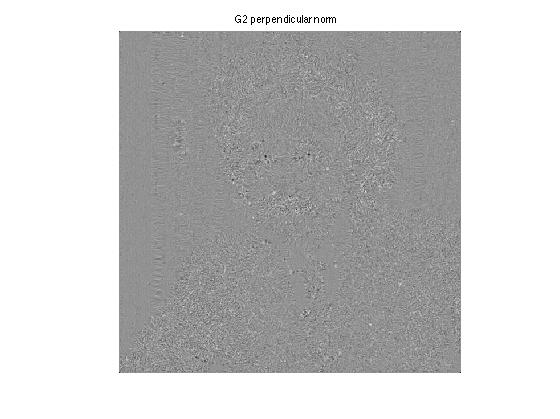
\includegraphics[width = 168pt, trim = 80pt 20pt 100pt 30pt, clip]{G2pn}
\newline
\tabT\tabT\tabT\tabT\tabT\tabT\tabT\tabT 
\tabT\tabT \textbf{G2}: dominant norm mean
\tabT\tabT \textbf{G2}: perpedicular norm mean
\newline
\tabT\tabT\tabT\tabT\tabT\tabT\tabT\tabT
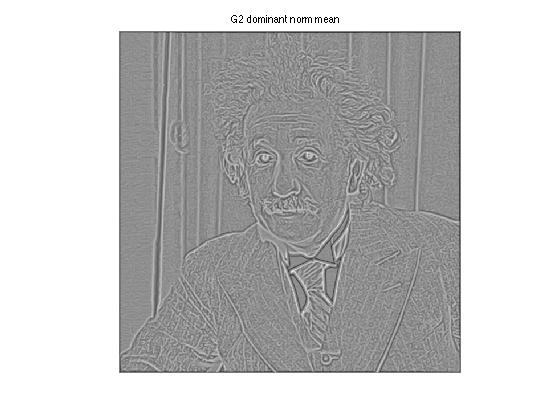
\includegraphics[width = 168pt, trim = 80pt 20pt 100pt 30pt, clip]{G2dnm}
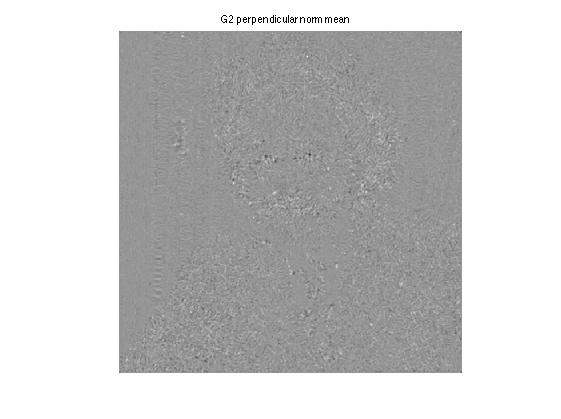
\includegraphics[width = 168pt, trim = 80pt 20pt 100pt 30pt, clip]{G2pnm}



\end{document}
